\section{Approach}
\label{sec:approach}

\begin{figure}%
	\centering
	\includegraphics[width=0.95\linewidth]{images/method_pipeline_1.pdf}
	\caption{Method overview.
		The input is a pair of equirectangular images, $I_t$ and $I_{t+1}$, and the output is the optical flow $\mathcal{F}_t$.
		The operators `$\oplus$' and `$\ominus$' rotate images forward and optical flow fields backward, respectively, using image warping (see \cref{sec:approach:warping}).
		The green box estimates the optimal rotation from a 360° optical flow field.
	}
	\label{fig:approach:pipeline}
\end{figure}

Our method comprises a global rotation warping and tangent-image-based panoramic optical flow method to mitigate the distortions in equirectangular image and the large displacements of pixels.
At the same time, our high-level approach generalises to any off-the-shelf perspective optical flow method, and thus will benefit from future improvements in optical flow methods.


As shown in \cref{fig:approach:pipeline}, our method comprises three steps:
(1)~We estimate the optical flow $\bar{\mathcal{F}}_t$ from ERP image $I_{t}$ to ${I_{t+1}}$, followed by rotating $I_{t+1}$ towards to $I_{t}$ based on the rotation estimate $\bar{R}$ from the flow $\bar{\mathcal{F}}_t$, which generates the warped ERP image ${\bar{I}}_{t+1}$ (see \cref{sec:approach:warping}).
(2)~We estimate the panoramic optical flow ${\hat{\mathcal{F}}}_t$ from $I_{t}$ to ${\bar{I}}_{t+1}$ based on cubemap projection optical flow (see \cref{sec:approach:projstit}), and then rotate the image ${\bar{I}}_{t+1}$ according to the rotation $\hat{R}$ estimated from the cubemap flow ${\hat{\mathcal{F}}}_t$ to generate ${\hat{I}}_{t+1}$.
(3)~We estimate the fine-scale flow $\tilde{\mathcal{F}}_t$ from $I_{t}$ to ${\hat{I}}_{t+1}$ using icosahedron projection optical flow (see \cref{sec:approach:warping}), then backward-rotate the fine-scale flow $\tilde{\mathcal{F}}_t$ by rotations $\bar{R}$ and $\hat{R}$ to generate the final 360° optical flow $\mathcal{F}_t$.
\looseness-1


Compared to perspective images, equirectangular images are continuous in all direction.
In \cref{sec:approach:definition}, we analyse and define the panoramic optical flow.
To solve the equirectangular image distortion, especially at the top and bottom, our method employs gnomonic projection to project the equirectangular image to tangent image~\cite{EderSLF2020}.
We use cubemap and regular icosahedron faces to uniformly sample the equirectangular image to solve this problem (see \cref{sec:approach:projstit}).
However, compared to a panoramic image, a tangent image has a smaller field of view, not larger than 180°, and just 90° for cubemap projection (without padding).
The tangent image optical flow operates on a pair of corresponding  tangent images from the same ERP image area,
which can fail when an object is only visible in one of the tangent images.
To compensate for the tangent images' narrow field of view, the global rotation operation is used on the target image $I_{t+1}$ to pre-align it with the source image $I_t$ (\cref{sec:approach:warping}).


\subsection{Definition of 360° Optical Flow}
\label{sec:approach:definition}

Spherical image coordinates are continuous in any direction on the image, e.g. pixel locations overflowing the image width will wrap around to the other side of the image.
If panoramic optical flow follows an object, a pixel's motion vector can fall outside the image boundary.
This is one reason that perspective optical flow methods cannot track pixels moving outside the equirectangular image boundary, because they do not support the horizontal coordinate wrap-around, as illustrated in \cref{fig:app:warparound}.
However, this introduces an ambiguity into 360° optical flow estimation, 
as there is more than one path from the source point to the target point along a great-circle on the sphere:
usually there is one shorter and one longer path.\footnote{One could also travel along the great circle a few more times, but these paths are getting longer and longer.}
To uniquely define 360° optical flow in the equirectangular image format, we define the optical flow to follow the shortest path from source to target along the great circle between them.
This naturally limits the maximum flow magnitude to $\leq$180°.



\begin{figure}[hbt!]
	\centering
	\subfigure[Source Image]{\includegraphics[width=0.26\linewidth]{images/wraparound/src_image.png}}
	\subfigure[Target Image]{\includegraphics[width=0.26\linewidth]{images/wraparound/tar_image.png}} 
	\subfigure[Perspective Optical Flow]{\includegraphics[width=0.26\linewidth]{images/wraparound/src2tar.png}}
	\subfigure[Wrap-Around]{\includegraphics[width=0.19\linewidth]{images/wraparound/wraparound.png}}
	\caption{\label{fig:app:warparound}%
		360° optical flow illustrated:
		A bunny moves from (a) to (b) within an ERP image.
		(c) Perspective optical flow methods estimate the bunny's motion from the right to the left via the front.
		(d) However, the shortest path for the bunny to move is along the back wrap-around.
	}
\end{figure}


\subsection{Projection \& Stitching}
\label{sec:approach:projstit}

To mitigate the distortions in ERP images, we locally undistort the ERP image to a perspective tangent image using gnomonic projection \cite{EderSLF2020}.
This way, we can apply any off-the-shelf perspective optical flow method directly on pairs of tangent images, first using a cubemap projection and later using an icosahedron projection to refine the 360° flow estimates.
In both the cubemap and icosahedron cases, we proceed as follows:
we first project the ERP image with gnomonic projection to generate 6 (cubemap) or 20 (icosahedron) perspective images that are tangent to the unit sphere;
we then use an optical flow method for perspective images to estimate optical flow for pairs of corresponding tangent images; and
finally, we stitch the optical flow fields for all tangent images back together in the ERP format.
Our approach in principle supports any perspective optical flow method, and results are therefore expected to improve as improved optical flow methods become available in future.

\vspace{-1em}
\paragraph{Gnomonic Projection.}
Like \citet{ZhaoYZLBT2020}, we use the gnomonic projection to produce tangent images.
These images are perspective images with the same camera centre as the ERP image, but their principal axis intersects the unit sphere at the tangent point with a circumscribed cube or icosahedron.
Depending on the choice and density of tangent points, tangent images cover different spherical surface areas, which determines the field of view (FoV) of the tangent images.
For estimating multi-scale motion and to uniformly sample the sphere surface, we select tangent points according to a regular cubemap and a regular icosahedron.
These are the most common convex regular polyhedra with 6 and 20 faces, respectively, and this results in different FoV with cubemap tangent images having a considerably wider FoV than icosahedron tangent images.
Therefore, cubemaps can estimate a larger motion vectors from the tangent images, although their angular resolution is coarser than the icosahedron's tangent images for the same spatial tangent image resolution.
To increase the FoV of tangent images and improve the continuity of optical flow at the boundary between tangent images, we add image padding to extend the area of tangent images, as illustrated in \cref{fig:approach:projection}.


\begin{figure}[hbt!]
	\begin{center}
		\subfigure[Gnomonic Projection]{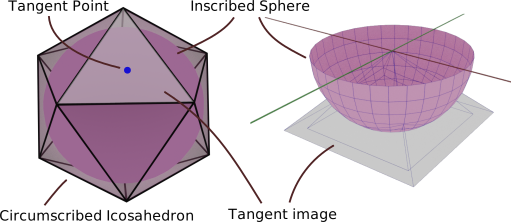
\includegraphics[width=0.57\linewidth]{images/tangent_image/tangent_image_7.pdf}}
		\subfigure[Target Image Padding]{\includegraphics[width=0.35\linewidth]{images/tangent_image/tangent_image.pdf}} 
	\end{center}
	\caption{\label{fig:approach:projection}%
		Tangent image projection and padding.
		(a)~Gnomonic projection maps points on the surface of a sphere from the sphere's centre to a point on the tangent plane.
		(b)~We add padding to the tangent images to extend their area and ensure overlap between tangent images.
	}
\end{figure}


\paragraph{Tangent Optical Flow Blending.}
As each tangent image's optical flow is estimated independently, the estimates might not be consistent in the overlap areas of adjacent tangent images.
When stitching the tangent flow fields in the equirectangular format, we thus compute a per-pixel blending weight $\omega_{i}$ for each tangent image $I_{t,i}$ to smoothly blend its optical flows $\mathcal{F}_{t,i}$ in the overlap areas.
The $\omega_{i}$ computes the colour difference between the source tangent image $I_{t,i}$ and the backwards-warped target image, to reduce the weight of badly estimated tangent images' optical flow $\mathcal{F}_{t,i}$.
The $\omega_i$ is estimated by 
$e^{-| I_{t,i} - Warp(I_{t+1,i}, \mathcal{F}_{t,i})|}$, the $Warp(\cdot , \cdot)$ is the backwards warping operation, and $I_{t+1,i}$ is the corresponding tangent image of $I_{t,i}$ at time ${t+1}$.
The $\mathcal{F}_t$ blended with the weighted tangent image optical flows,  $\frac{\sum_i{\mathcal{F}_{t,i} \cdot \omega_{i}}}{\sum_i{\omega_i}}$.




\subsection{Global Rotation Warping}
\label{sec:approach:warping}

Inspired by warping-based optical flow~\cite{BroxBPW2004}, we estimate the global rotation to pre-align the ERP image $I_{t+1}$ to $I_{t}$.
This helps reduce the range of pixel motion to a level that is more suitable for the smaller FoV of tangent images.
We compute the global rotation $\bar{R}$ from the computed optical flow field as follows.
First, we convert the coordinates of the start and end points of all optical flow vectors to spherical coordinates with unit length.
Then, we solve for the optimal rotation between the start points and the corresponding end points using least-squares fitting, which can be solved in closed form by singular value decomposition \cite{ArunHB1987,SorkiR2017}.

\vspace{-1em}
\paragraph{Global Rotation Image Warping.}
After estimating the global rotation $\bar{R}$ from the 360° optical flow, we warp the target image $I_{t+1}$ by the rotation $\bar{R}$ to align it to the source image $I_{t}$. %
We apply global rotation warping based on the coarse to fine principle.
First, we estimate the rotation $\bar{R}$ directly from ERP optical flow to roughly align the image $I_{t+1}$ and compensate for camera ego-motion.
We then use the cubemap optical flow to estimate the residual rotation $\hat{R}$ to fine-tune the global rotation alignment.

\vspace{-1em}
\paragraph{Global Rotation Optical Flow Warping.}
To recover the final 360° optical flow field $\mathcal{F}$ from the icosahedron optical flow $\tilde{\mathcal{F}}$, the end points of $\tilde{\mathcal{F}}$ need to align with the pixel position in the input image $I_{t+1}$.
When estimating the optical flow, only the target image $I_{t+1}$ is rotated, so we now need to rotate the end points of $\tilde{\mathcal{F}}$, i.e $\tilde{\mathcal{F}}^\text{EP}$, in the opposite direction.
To `rotate' an ERP pixel, we first convert it\new{s ERP image coordinates $\mathbf{x}$} to Cartesian 3D coordinates using \new{the inverse projection operator} $\mathcal{P}^{-1}$, rotate it about the centre of the sphere, and then convert it back to ERP \new{image coordinates} using $\mathcal{P}$.
Applied to optical flow, this yields:
\begin{equation}\label{equ:approach:globalwarp}
	\mathcal{F}(\mathbf{x})
	= \mathcal{F}^\text{EP}(\mathbf{x}) - \mathbf{x}
	= \mathcal{P} \left( \hat{R}^\top \cdot \bar{R}^\top \cdot \mathcal{P}^{-1}(\tilde{\mathcal{F}}^\text{EP}(\mathbf{x}))\right)  - \mathbf{x}
	\text{.}
\end{equation}
